
\section{Missing transverse energy decomposition using the
  event thrust axis }
Rather than using the nominal $\exmiss$ and $\eymiss$ along the nominal
geometrical reference frame of the detector one can define a reference
system that is connected to the event and its kinematics~\cite{CMS:AN-2009-025}.  We use the
tracking system of CMS to define a reference system for the
decomposition of the $\etmiss$ as follows:

\begin{itemize}
\item use the leading track transverse axis (as in for example~\cite{CMS:PAS-EWK-008-06}).
\item use the Transverse Thrust (TT) axis, calculated using only tracks. This
  is the axis of the  highest transverse momentum aligned along it
  (calculated event by event) as follows:
  \begin{equation}
    \mathrm{TT} = \max_{\phi_\mathrm{TT}}\frac{\sum_{i}|p_\text{T}^{i}\cos(\phi_\mathrm{TT}-\phi_{i})|}{\sum_{i}p_\text{T}^{i}}
  \end{equation}
\end{itemize}

We use only ``high-purity'' tracks in the above determinations of the
axes. When there is calorimetric activity due to particles produced in
the collisions, it is more likely to be along these ``physics
preferred axes''. This is demonsrated in Figure ~\ref{fig:MET-TT}
which shows the $\etmiss$-TT directional correlation for events collected at
$\sqrt{s}=900$ and $\sqrt{s}=2360$ GeV compared with the corresponding
Monte Carlo simulation.  Similar behavior is observed if instead of the
TT-axis the leading track axis. In this section we use the TT-axis
being the better physics motivated one in minimum-bias events.

\begin{figure}[h!]
 \centering
 \begin{tabular}{ll}
   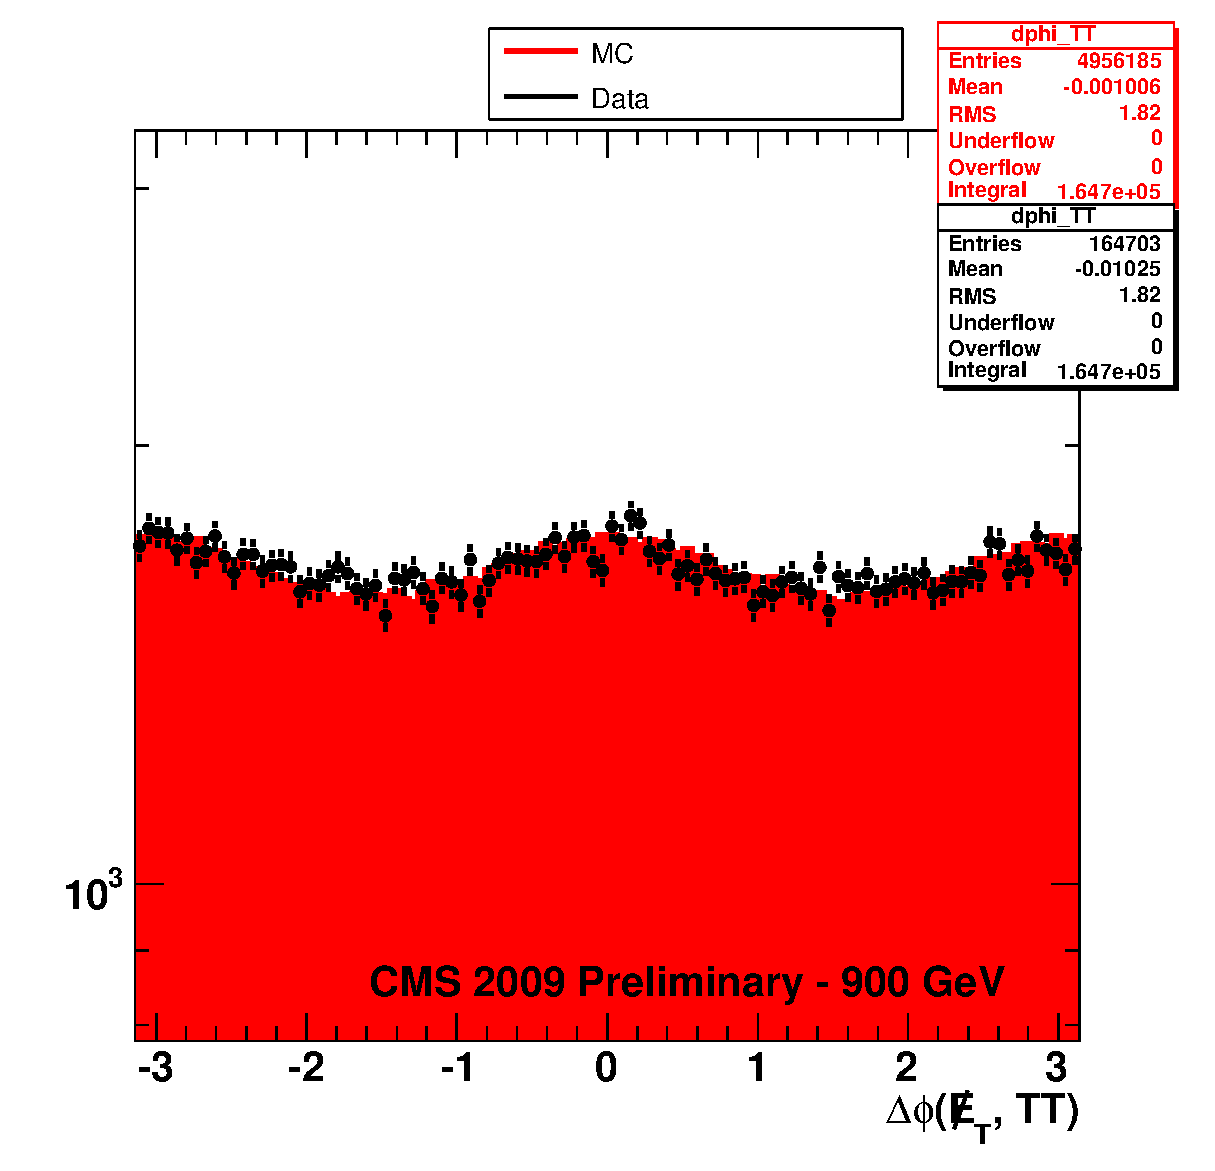
\includegraphics[width=0.5\textwidth]{plots_DataVsMC_MB_900GeV/dphi_TT_900.eps}&
    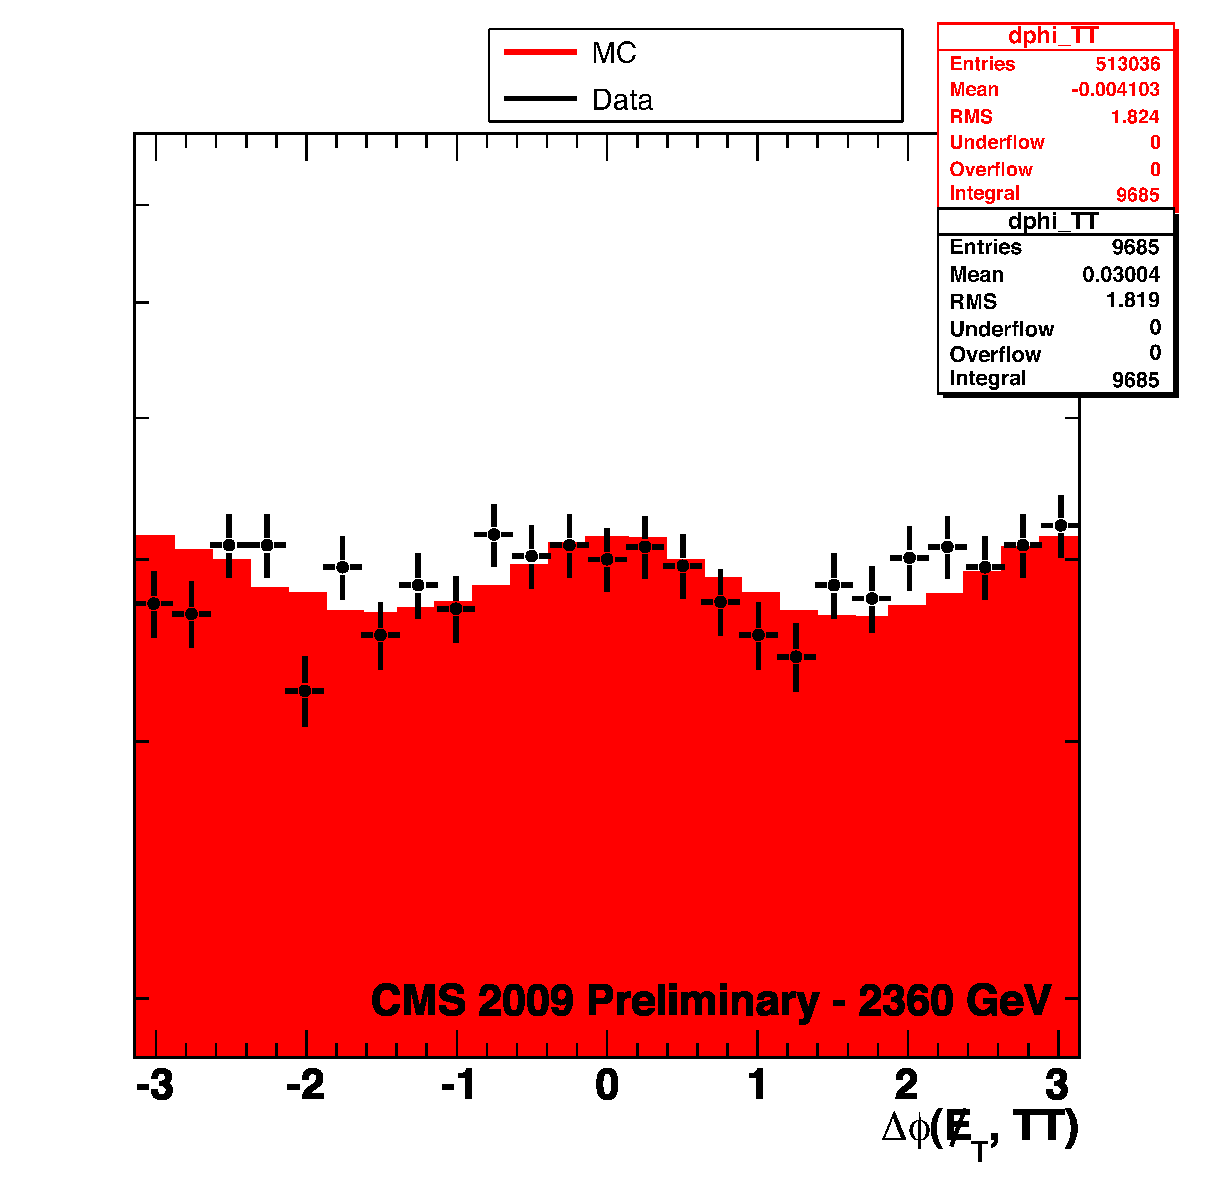
\includegraphics[width=0.5\textwidth]{plots_DataVsMC_MB_2360GeV/dphi_TT_2360.eps}\\
 \end{tabular}
    \caption{$\Delta\phi$ between the transverse thrust axis and the
      $\etmiss$ direction for events collected at $\sqrt{s}=$900 GeV
      $\sqrt{s}=$2360 GeV and comparison with the corresponding Monte
      Carlo Simulation.  A weak correlation between these two axes is
      observed (as expected) while the dominant component is due to
      noise.
      \label{fig:MET-TT}}
\end{figure}

The $\etmiss$ in the min-bias events analyzed is
decomposed into two orthogonal components, denoted $\etmiss_\perp$ and
$\etmiss_\parallel$ and corresponding to the $\etmiss$ components
perpendicular and parallel to the transverse thrust axis direction
respectively:
\begin{equation}
{\rm \etmiss}_{\parallel} = \vec\etmiss\cdot
\vec{p}_\text{T}^\mathrm{TT}/|\vec{p}_\text{T}^\mathrm{TT}|~~,
    ~~ {\rm \etmiss}_{\perp} =
\sqrt{|\vec\etmiss|^{2} -
|\rm{\etmiss}_{\parallel}|^{2}}
\label{eq:U}
\end{equation}

 $\etmiss$ denotes the raw (uncorrected) calorimetric missing
 transverse energy
 
The corresponding components resolution are  shown in 
 Fig.~\ref{fig:MET-res-900} for $\sqrt{s}=900$ GeV  and
 Fig.~\ref{fig:MET-res-2360} for $\sqrt{s}=2360$ GeV.

\begin{figure}[h!]
 \centering
 \begin{tabular}{ll}
   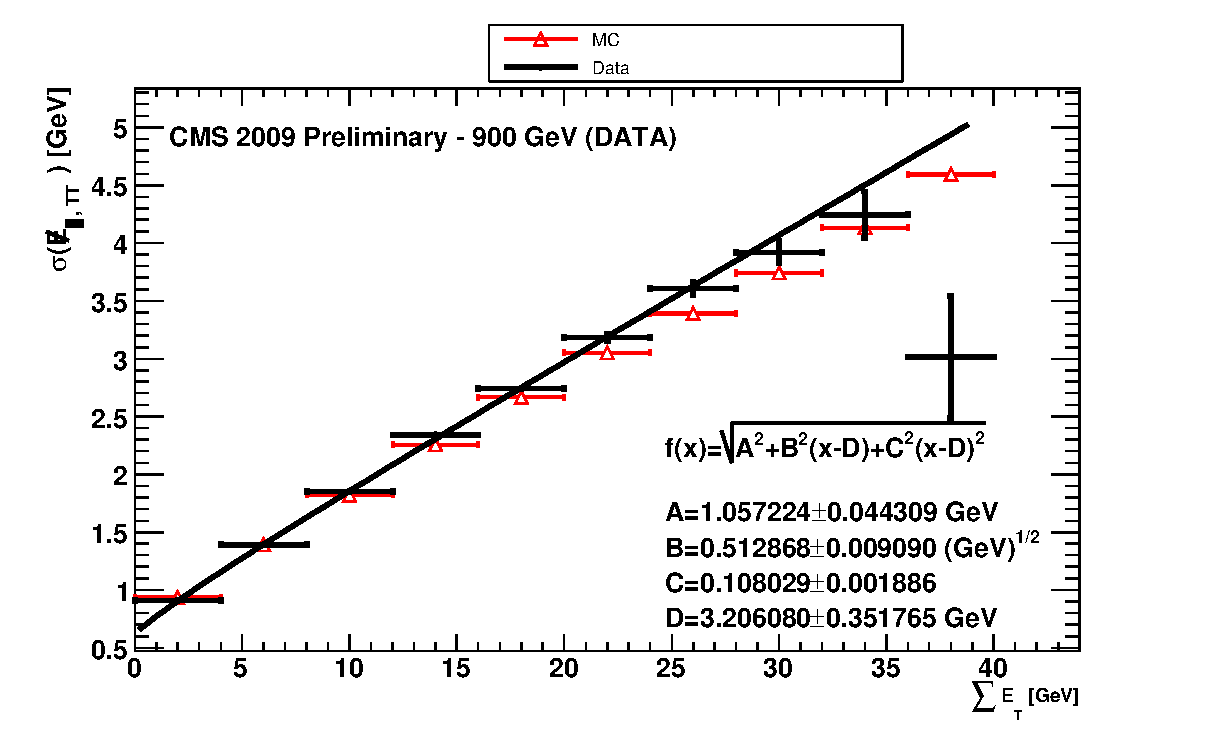
\includegraphics[width=0.5\textwidth]{plots_DataVsMC_MB_900GeV/DATA_METpar_TT_sigma_900.eps} &
    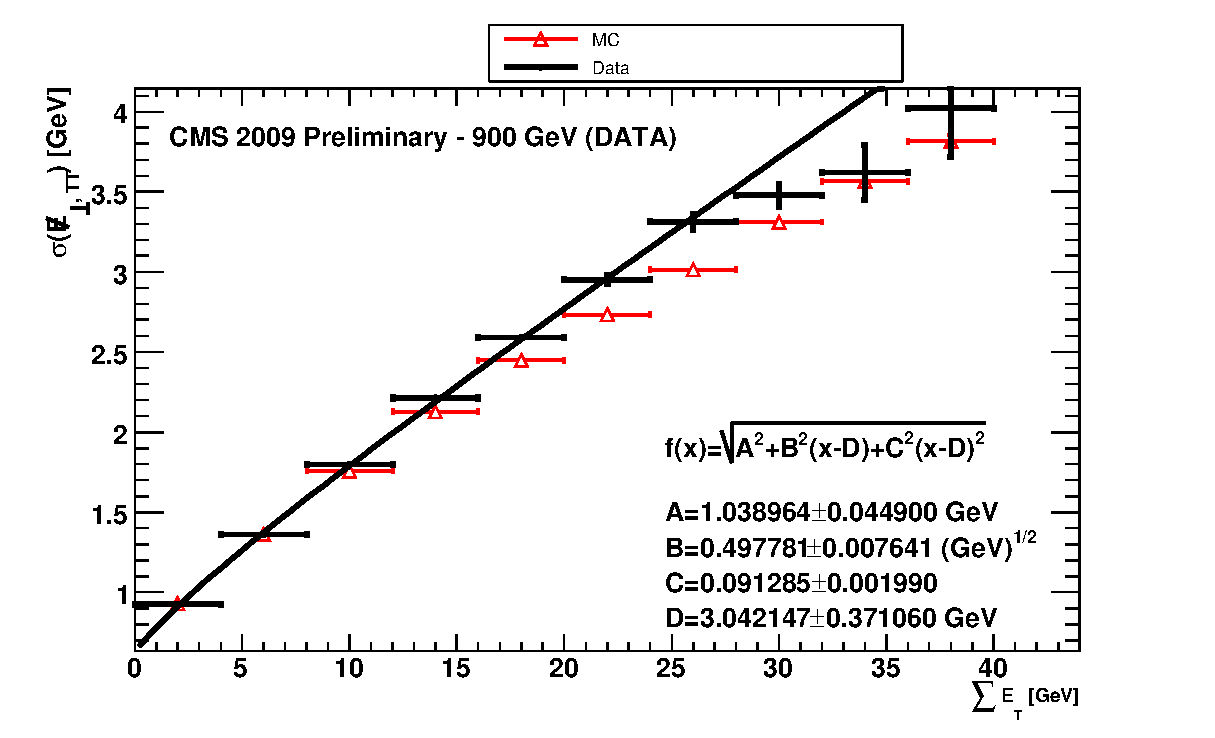
\includegraphics[width=0.5\textwidth]{plots_DataVsMC_MB_900GeV/DATA_METperp_TT_sigma_900.eps} \\
\end{tabular}
\caption{ Resolution of $\rm{MET}_{\parallel}$ and ${\rm
    MET}_{\perp}$  as a function of the scalar sum of energy in all
  the calorimeters. Events collected at $\sqrt{s}=900$ GeV and
  comparison with MC. The fit corresponds to the data distribution.
  \label{fig:MET-res-900}}
\end{figure}

\begin{figure}[h!]
 \centering
 \begin{tabular}{ll}
   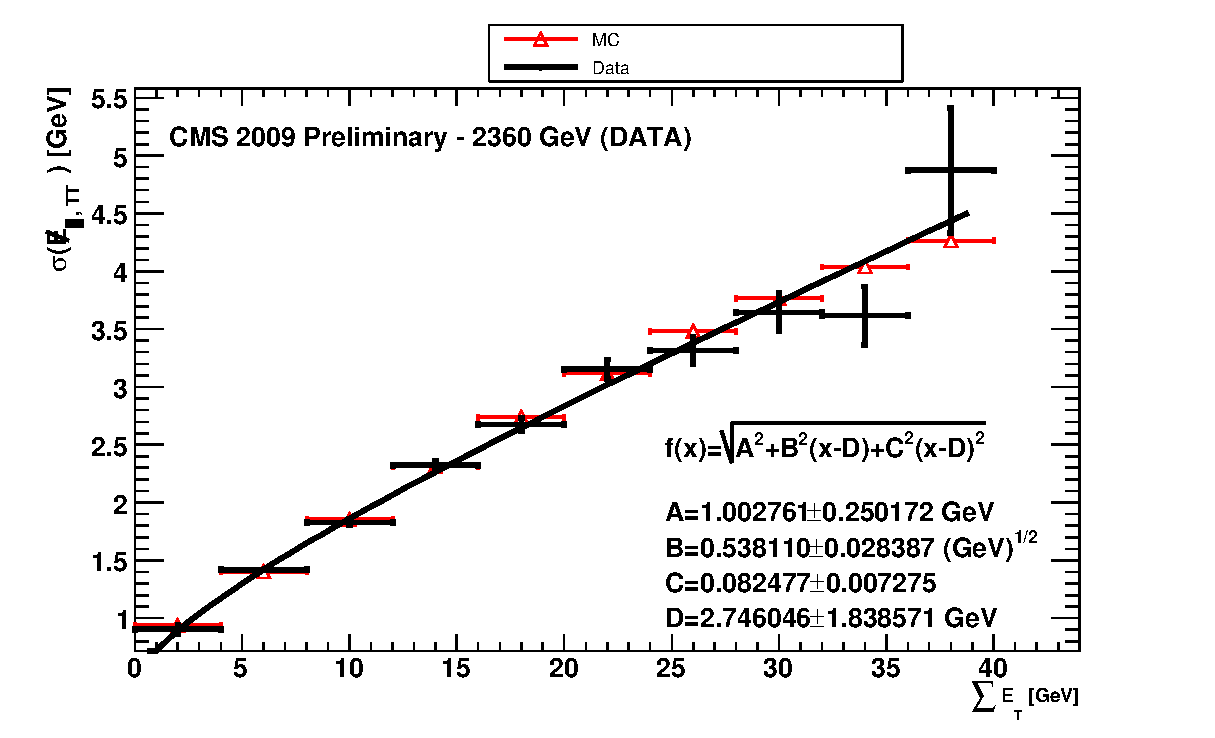
\includegraphics[width=0.5\textwidth]{plots_DataVsMC_MB_2360GeV/DATA_METpar_TT_sigma_2360.eps} &
    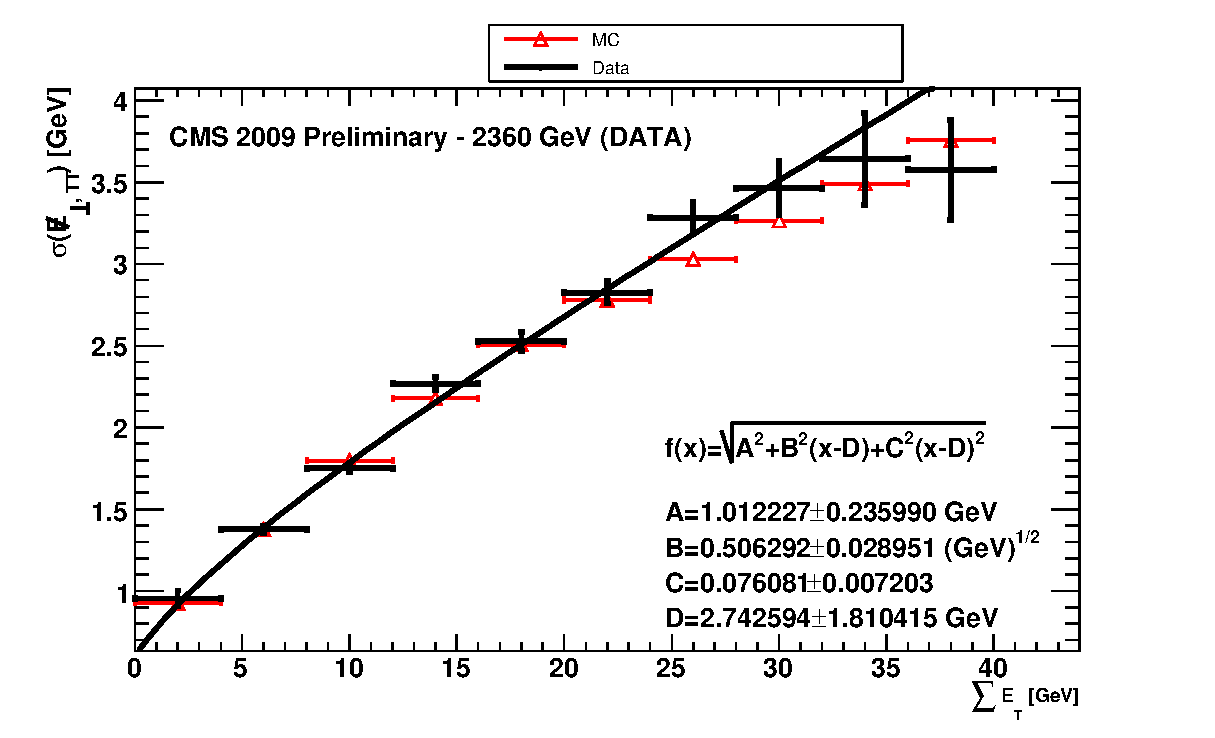
\includegraphics[width=0.5\textwidth]{plots_DataVsMC_MB_2360GeV/DATA_METperp_TT_sigma_2360.eps} \\
    \end{tabular}
 \caption{ Resolution of $\rm{MET}_{\parallel}$ and ${\rm
     MET}_{\perp}$  as a function of the scalar sum of energy in all
   of the calorimeters. Events collected at $\sqrt{s}=2360$ GeV and
   comparison with MC. The fit corresponds to the data distribution.
\label{fig:MET-res-2360}}
\end{figure}

\clearpage

